\documentclass[10pt,twocolumn]{article} 

% use the oxycomps style file
\usepackage{oxycomps}

% read references.bib for the bibtex data
\bibliography{references}


% include metadata in the generated pdf file
\pdfinfo{
    /Title (The Occidental Computer Science Comprehensive Project: Comparing Food Delivery Costs Amongst the Most Popular Delivery Apps)
    /Author (Xintai Aaron Ao)
}

% set the title and author information
\title{The Occidental Computer Science Comprehensive Project: Comparing Food Delivery Costs Amongst the Most Popular Delivery Apps}
\author{Xintai Ao}
\affiliation{Occidental College}
\email{xao@oxy.edu}
\begin{document}
\maketitle

\begin{abstract}
This paper is the final paper outlining my Occidental College Computer Science Comprehensive Project (COMPs): \textit{Comparing Food Delivery Costs Amongst the Most Popular Delivery Apps}. This paper begins by introducing this project's problem context. Next, it address the technical aspects of realizing this work. This paper also addresses lingering ethical concerns. Replication instructions and an overview of the code developed in this work for future users to engage with this project have been included as GitHub README documents in addition.
\end{abstract}

\section{Problem Context}

For my Occidental Computer Science Comprehensive project, I want to build a web application that can help consumers compare the prices of the "Big Four" food delivery applications: UberEats, Postmates, Grubhub, and DoorDash. The goal of this project is to build a fully functioning web application that would eliminate a common problem among people that order food through delivery apps: the hassle of checking multiple delivery apps just to compare their respective pricing for one food order. Essentially, what should attract people to this web application is its ability to save time and money by eliminating the process of having to go through each online delivery app on one's phone just to save a few extra dollars. This web is meant to increase the efficiency in which a user can optimize their delivery experience and maximize their money and eliminate concerns regarding restaurant exclusivity to certain delivery apps. 

For the scope of this project, I will be focusing on restaurants within a 15 mile radius of Occidental College. This range of potential restaurants encapsulates the scope of this project as it will be a group of restaurants that the average person at Occidental College will most likely order from, which includes students and staff alike. According to a study conducted by \citetitle{ResearchGate}, the main demographic of delivery app users looking to save money are students below the age of 20 and are more prone to choose a delivery app that offers more coupons or special-time offers. Though the intended demographic for this project are people with strict budgets or lower incomes such as high school and college students, this web application can still be useful for people that have the general need to save money while ordering food online. The goal of this project is to make food delivery more accessible for people on a budget whilst saving them time and money. 

The most reasonable scope for this comprehensive project would be to build a web application that solely focuses on comparing the food item prices between two major food delivery applications: UberEats and GrubHub. Other delivery applications could also be added into this comparison web application in the future, including DoorDash, Postmates, InstaCart, Yelp, goPuff, and et cetera. Delivery fees and times are listed separately in the resulting lists from the user input. A problem that arises with this comprehensive project is the task of collecting real-time and history data from these major online delivery conglomerates. Though the historical and real-time data from these applications are not readily available to the public, there is a solution to this: web scraping. By web scraping data from these food delivery apps and storing them in a database, I can then accurately determine the differing price points revealing to the user what the best deal would be. This project will not run into any legal issues so long as the intended web application will not be sold for the purpose of monetary gain.

\begin{figure}
    \centering
    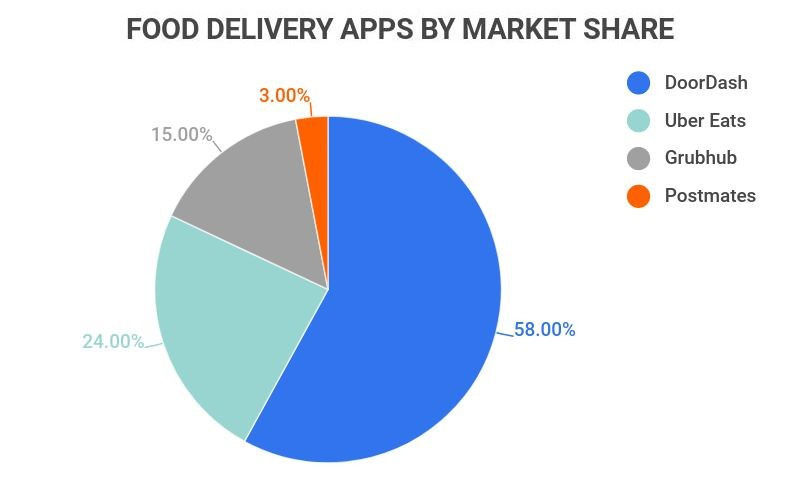
\includegraphics[width=.98\linewidth]{COMPS Final paper/Delivery Market.jpeg}
    \caption{
        Saturation of Online Food Delivery Market
    }
    \label{fig:second-page}
\end{figure}

This project will be very useful for the average consumer as it will give them the access to a convenient tool that will save them time and money. This project benefits the average delivery app user as this web app will give them the ability to save money on commonly used service other than through coupons or special limited time deals on the apps. However, this web app has implications to be potentially detrimental for online food delivery businesses; consumers would reap the benefits of saving money on online food deliveries at the expense of these conglomerates. If this project were to be expanded so that a consumer could order and pay without having to change apps, then it could potentially even steer consumers towards specific applications that would offer the best deals, increasing competition amongst delivery apps. However, in the limited time for this project, I will focus on the price comparison component rather than a creating dual functioning food delivery and price comparison web.

\begin{figure}
    \centering
    \includegraphics[width=.98\linewidth]{COMPS Final paper/Covid.jpeg}
    \caption{
        Financial Effect of Covid-19 on Online Food Delivery
    }
    \label{fig:second-page-1}
\end{figure}  

\section{Technical Background}

For this comprehensive project, the overall stack for the web application is going to be: the user enters the food item they want to order into the web application. Some food items the user can choose include "burritos", pad thai", "burgers", and et cetera. Then the app finds and returns two lists of the respective restaurants within the user's general vicinity. Next to each restaurant name will be listed a food item most closely related to the users search item along with its price, delivery time, and delivery fee. If the user enters an invalid search item, rather than a resulting list, a message will pop up explaining their search did not return any results.

For this project, the method in which real-time data will be extracted from UberEats and GrubHub will be through web scraping. As explained in the article \citetitle{WebScraping}, web scraping is the automated retrieval of data from the text of a web with the aid of bots and storing said data in a structured format. 

With the onset of Covid-19 and the subsequent rapid increase in users of online-to-offline food delivery service, the online food delivery market has become largely saturated. According to \citetitle{Saturation}, there have been both major positive and negative impacts on the online delivery market: the positive effect is that the pandemic has provided a suitable condition for online food delivery companies to promote their services. The negative impact that the pandemic has had on the online food delivery market is that it has triggered "the acceleration of market saturation and reduce the market potential". This has led artificially inflated menu pricing from specific restaurants and the addition of hidden fees and costs to both the restaurants and consumers of the online delivery market.

This project aims to prevent consumers from having to deal with these predatory behaviors from major food delivery app companies by finding them the best deals possible. In doing so, the hope for this project is to potentially reinvigorate a largely saturated market. The convenience of ordering food online has ironically become a hassle in itself for a large number of consumers, especially for those still in school or on a budget. 

For the back-end portion of my web application project, I opted to use the LAMP stack for my database and code because it allows for real-time access to data in an efficient manner. The SQL files will be uploaded to a MySQL database (phpMyAdmin) and can be accessed quickly by my website. To build a responsive web app, LAMP is one of the popular tech stacks, but other options such as MEAN or MERN exist. I chose LAMP due to my prior knowledge of PHP and the time constraint of the project. This made LAMP the simplest and quickest choice to implement.

The SQL files in the database will contain information about various restaurants obtained from UberEats and GrubHub. The information contained in these files includes Restaurant Name, Address (as a unique key), Dish Name, Dish Price, Delivery Fee, and Delivery Time. The "Restaurant\_name" is used as the primary key to link the different tables in the relational database, allowing for efficient querying of multiple tables to generate useful information. The address was added as a unique identifier for restaurants with multiple locations in the vicinity of Occidental College.

For this project, LAMP stack (Linux, Apache, MySQL, PHP) was chosen as the tech stack for this web app due to its efficiency in real-time data access and the developer's prior knowledge of PHP. The database consists of two separate SQL files with variables like restaurant name, address, dish name, dish price, delivery fee, and delivery time. PHP is used to retrieve the restaurant data from the database and render it in the front-end. The front-end, initially created in Webflow, was converted into PHP to allow for dynamic content and additional functionality using JavaScript. Hostinger was used for testing and debugging the software.

To test and debug the web application, I used Hostinger as the web hosting platform. The process of testing involved entering random user inputs and checking if the variables or arrays were correctly displayed. If I encountered any problems, I would look for a solution by identifying the issue, such as the issue with non-related searches appearing when a multi-word user input was entered, which was resolved by making changes to the SQL code in the file responsible for outputting the results. This approach allowed me to identify and resolve any issues with the web application and ensure that it was functioning as intended.

\section{Prior Work}

Some prior work that has been done to solve similar issues in the online food delivery market are the delivery price comparison apps “Mealme”  and “FoodBoss”.

Mealme is an iOS app that has features similar to what I want in my web application. A breakdown of MealMe: the iOS app first allows the user to set a specific price range for their desired food delivery order. Next, the app will display multiples lists that fit into the consumer's price range including trending items, daily deals, popular restaurants, cheapest deliverable food and drink options, and so forth, all relative the user's location. One problem with this application is that it is only available on iOS. That is why I plan on creating a web application so that it may be available for all users, as long as they have access to a computer or cell phone. I will not try to emulate all the components of Mealme since the problem in doing that would essentially be me trying to recreate an app that hires hundreds of thousands of dollars worth of coders in salary, within four months. That would become a far too complicated task to complete for the given timeline for this project.

The Mealme claims that the app uses “A.I.” to find the best deals possible for its users, which is not true. What the app does do is it web scrapes data from these major delivery company's apps and presents them in a comprehensible way to its users. However, the app’s interface is not fluid, in that it takes a long time to load, and it occasionally does not display a specific delivery service option for a food order. This leaves room for errors such as longer than expected delivery times, missing orders, and inaccurate delivery fee calculations, such as the negligence of hidden service fees unique to each major delivery app.

According their main website, Foodboss is essentially the Kayak for food delivery services, in that it compares the delivery prices of nearby restaurants. This application's function is the most similar to what I want to do for this project. However, similar to MealMe, the application is only available on the IPhone whereas I want to create a web that is available to all users.

Though this app is most similar to what I want to emulate, for the given timeline and scope of this project, trying to create a web with all the components of MealMe would be a far too daunting and complicated task to complete. However, for the timeline of this project, the most reasonable scope would be to build a web application that solely focuses on comparing the total cost of a set online delivery orders from the four major delivery applications. Delivery fees and taxes will be included into the total cost of each delivery app.

\begin{figure}
    \centering
    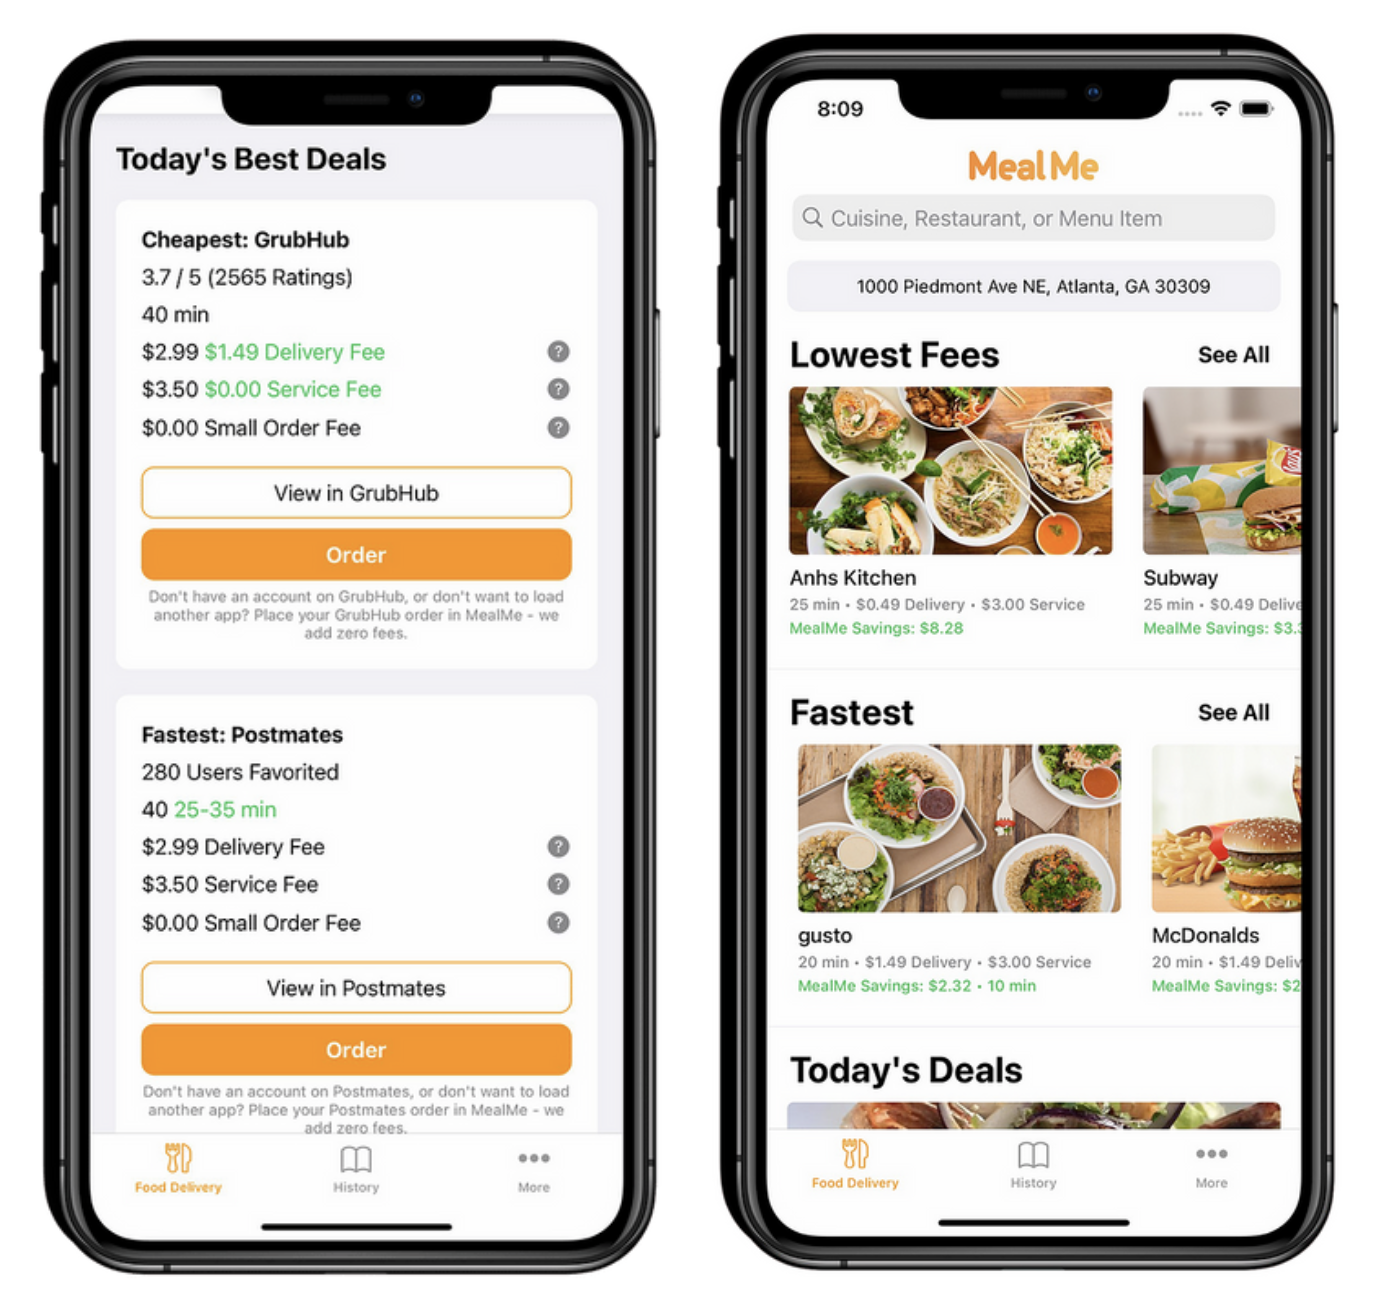
\includegraphics[width=.98\linewidth]{COMPS Final paper/Mealme.png}
    \caption{
        MealMe Interface
    }
    \label{fig:second-page-2}
\end{figure}

\section{Methods}

For this COMPs project, I used the cloud-based web data extraction tool Octoparse because it is free and it also enables users to scrape unstructured data from major applications including that of the major food delivery services. Octoparse can save this data in different formats including through Excel, HTML, and CSV files, which will be necessary for this project. For the purpose of this project, I will be extracting the data into CSV files to then later convert into SQL files, which is more applicable in the case of creating a web app. This data scraping and formatting would otherwise be difficult or near impossible within the given time frame of this project. This is because the extraction of data from these major corporation web applications would be impossible since they are dynamically generated and are formatted based on the cookies of the user logging into the web page. Also, without the legal and written consent of these companies, extracting this data could be illegal. Also, I would need to create my own bots and find a way to illegally extract data from the these major corporation website apps. Though I do not mind ripping off major corporations, for the sake of this project and the amount of time given to complete it, this would be completely impossible and unnecessary.

\begin{figure}
    \centering
    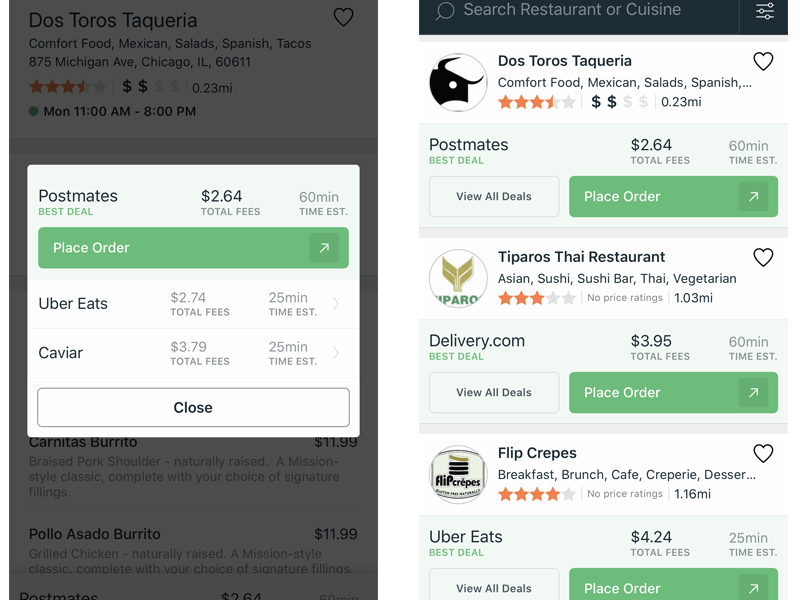
\includegraphics[width=.98\linewidth]{COMPS Final paper/FoodBoss.png}
    \caption{
        FoodBoss Interface
    }
    \label{fig:second-page-3}
\end{figure}

For this comprehensive project, since I plan to utilize web scraping to pull real-time data from the UberEats and GrubHub, the main application stack for this web application project is: How do I want users to interact with this website? 

The goal for this web application at its core is to give its users the ability to aggregate and compare prices between major food delivery apps. The best way to do this is by designing the web application so that it functions similarly as to how a major food delivery app would.

First, the web application would need to have a search bar for specific food items so that the user can search for what they want. In this web application, when a user searches for a restaurant, the order in which the application should work is:

\begin{enumerate}[label=(\Alph*)]
\item The user enters their desired food item.
\item The web app outputs two resulting lists, one for UberEats and one for GrubHub.
\item Each resulting listing list will include the resulting food item name, restaurant name, food item price, delivery fee, and deliery time.
\item If a specific delivery service is not available for that particular restaurant or specific order, then the output on the list will be labeled as "Not Available".
\end{enumerate}

Since UberEats and GrubHub are both dynamically generated and formatted based on the cookies of the user logging into the web page, the method which I will use to scrape each delivery app will have to be tailored to each. The web scraping will all done through Octoparse as the tool allows for custom scraping on different website formats and types of data. The data extracted from these major food delivery websites will first be formatted into CSV files which then will be converted into SQL files using an online converter. 

\begin{figure}
    \centering
    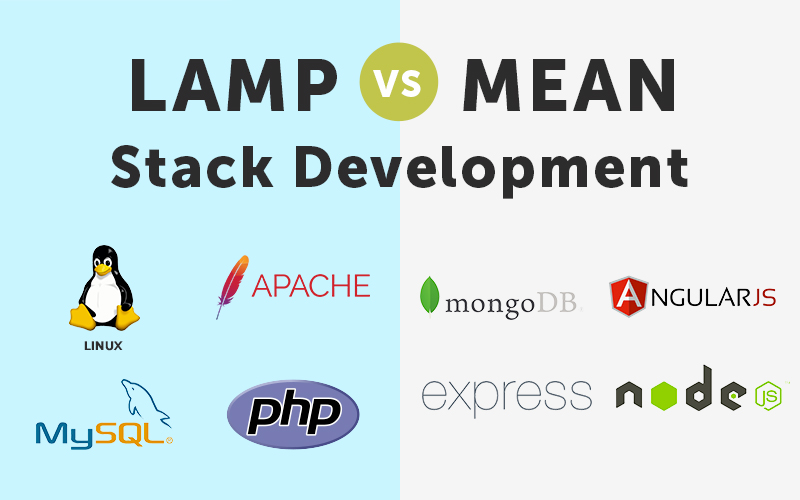
\includegraphics[width=.98\linewidth]{COMPS Final paper/LAMP.png}
    \caption{
        LAMP stack vs MEAN Stack
    }
    \label{fig:second-page-3}
\end{figure}

\subsection{Software Development}

For both my database and code, I primarily chose to use LAMP stack as that would be the most efficient way for my website to access the data in real time; the SQL files would be uploaded into a MySQL database (phpMyAdmin) from which my website will be able to access the multi-variable data contained within them in a sub-half second. For building a responsive web app, several popular tech stacks similar to LAMP stack exist. A dynamic web app is needed to have all the desired features, and common options for this also include MEAN and MERN stacks. However, due to the time constraint of the project and my prior knowledge of PHP, I chose to use LAMP stack, making it the simplest and quickest option to implement.

Within the database will have two separate and unique SQL files containing the essential information scraped from UberEats and GrubHub based on these variables: Restaurant Name, Address (unique key), Dish Name, Dish Price, Delivery Fee, and Delivery Time. The address was a necessary addition as a unique identifier for the restaurants that had multiple locations within the area near Occidental College. All of these variables are connected in a relational database by their “Restaurant\_name" as their primary identifying key. Since MySQL uses primary keys to link different MySQL tables, this allows different tables to be queried at once to generate useful information. 

In order to retrieve the restaurant data based on user input and then render that into its proper location in the front-end, PHP would have an appropriate application due to this web app's use of LAMP stack. PHP also allows for the retrieval of the restaurant data which is stored in the back-end of the web app and then render PHP content to contain data from MySQL which essentially allows me to create a fully functional web app. Since I created the front-end interface in Webflow, I redesigned them to be in PHP: I converted my static HTML pages generated from Webflow into PHP to generate dynamic content with the front end components that I created in Webflow. PHP also allows the use of JavaScript in PHP files which was very useful for both generating dynamic content but also for adding functionality.

All of the testing and debugging of my software was done through Hostinger, a web hosting platform where I am hosting all the necessary files for my web application. Whenever I would run into a problem, the process in which I would follow would be enter a random use input to see if any variables or arrays were not being displayed or if the information was correct. For example, an issue that took me a while to fix was when a multi-worded user input was put into the website, non-related searches would often be displayed. This issue turned out to be a simple SQL coding fix in which I simply changed a few lines of code within the file responsible for outputting results to user input.

\begin{figure}
    \centering
    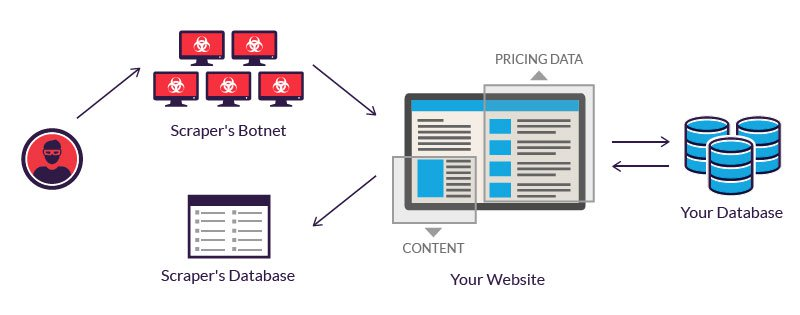
\includegraphics[width=.98\linewidth]{COMPS Final paper/What is Scraping.jpeg}
    \caption{
        How Web Scraping Works
    }
    \label{fig:second-page-4}
\end{figure}

\section{Evaluation Metrics}

In order to properly evaluate my senior comprehensive computer science web application project, I would have to consider the following basic aspects:

\begin{enumerate}
    \item Functionality: Does the application meet the requirements and specifications defined for the project? Does it perform its intended functions correctly and efficiently?
    \item User Experience: Is the application user-friendly, easy to navigate, and visually appealing? Does it provide a positive user experience?
    \item Performance: Does the application perform well under normal and heavy loads? Is it fast, responsive, and scalable?
    \item Code Quality: Is the code well-organized, readable, and maintainable? Does it follow industry-standard coding practices and best practices for web development?
    \item Documentation: Is the project documentation thorough and complete? Does it include a detailed description of the application's features, design, and architecture, as well as instructions for installation and use?
    \item Testing: Has the application been thoroughly tested to ensure that it meets all requirements and functions correctly?
    \item Innovation: Does the application bring something new and innovative to the field or solve a problem in a unique way?
\end{enumerate}

One way I set out to evaluate the effectiveness of my web application thoroughly was through the utilization of guided observations and anonymous survey questions. This would cover all the basics of the questions above. This is similar to what others in the software development field have used to evaluate the effectiveness of problem-solving software and technology. One example of this can be seen in the field evaluation portion of a published research paper about the effectiveness of a new software design that attempts to solve the existing problem of lack of integration of  Intelligent Decision Support into Critical, Clinical Decision-Making Processes despite Intelligent Decision Support systems already existing \cite{unremarkableAI}. This research paper describes researchers trying to create a new system that Doctors and other medical professionals could utilize in real life. The authors of this paper aimed to address the issue of doctors not using existing Intelligent Decision Support systems, due to dissatisfaction with them. They designed a new system that considered the identified flaws in current platforms and user-specific needs. To assess its effectiveness, they employed a combination of user observations and interviews.

Similarly, the aim of my delivery comparison web application is to address the dissatisfaction with the current prices available on the market. This new app is designed to address the flaws in existing apps and meet user needs. The effectiveness of the app will be evaluated through a similar method of user observations and interviews, with the hope of providing a faster and simpler way of discovering new places and encouraging people to go out more.

The main goal in testing this project is to evaluate whether or not this web application functions as intended. The important aspects of this web application worth testing is:

\begin{itemize}
    \item Is the app convenient to use? Will have beta testers test that.
    \item Is the web application intuitive?
    \item Is the outputted information correct?
    \item Is the output list load time sub-half second?
    \item Are there any abuse cases? Meaning does it work under the corner cases? 
    \subitem Example cases: UberEats doesn't exist; user inputs fake restaurant or items; data feeds become corrupted; i.e. anything in which the processing deviates from normal operations.
    \item How does the web application handle these deviations? How can they be corrected?
\end{itemize}

During testing and the designing of this web app, I found that entering a set number of orders from different restaurants into the web application was initially the best of way of evaluating its efficiency. Each of the orders were unique in that they each contained different food items or drinks and that they will be from specific restaurants. Some of the order sets purposefully contain fake items, an inordinate amount of one item, or items not available at any of the restaurants within the vicinity of Occidental College.

The best way to evaluate how well this web application project could save money for potential users is through user testing; the testers for this project included students from Occidental College and surrounding Colleges, which age group was the main focus group. Since these people are the main demographic for this project, only they would be the most suitable testers to earn feedback from. An important aim for this project is the feeling on convenience and lack of frustration for these users. I do not want this web application to feel as if it is an extra unnecessary step for an action as simple as ordering food through an app. I would consider the web application a failure if and only if it fails to save its users money less than 50\% of the time or if it becomes more of an inconvenience than just checking multiple delivery apps for the best deal.

\begin{figure}
    \centering
    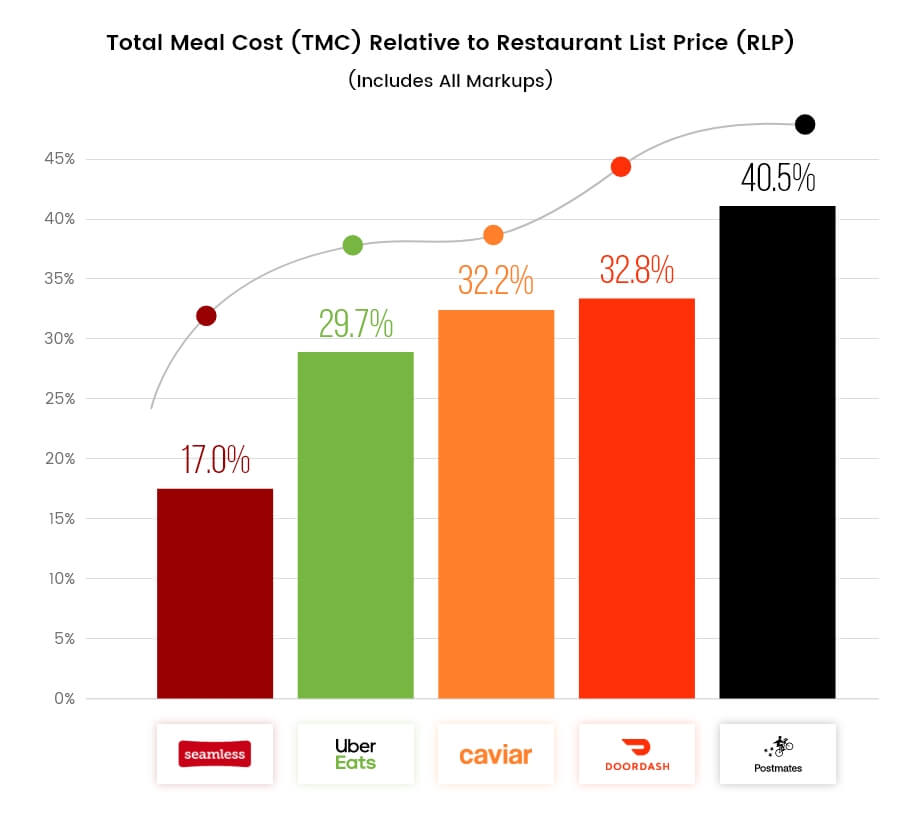
\includegraphics[width=.98\linewidth]{COMPS Final paper/TMC.jpeg}
    \caption{
        How Much Extra Customers Pay per App
    }
    \label{fig:second-page-5}
\end{figure}

\section{Results and Discussion}

Though my web application was successful in finding users a compiled list of the cheapest food delivery options from two major food delivery companies relative to Occidental College, I was not able to fully complete every goal as initially intended in the beginning of the semester. To reiterate, the intended goal of this project was to be able to compare a comprehensive list of different delivery options of four major food delivery companies for restaurants relatively close to Occidental College. This goal was not completely achieved due to the limited time frame and difficulties that occurred with figuring out individualized web scraping for each delivery app during the time of this project; the extraction of data from these major corporation web applications would require bots to scrape sites that are dynamically generated and formatted based on the cookies of the user logging into the web page. However, the final web application was still a success in regards to compiling two comprehensive lists of food delivery options for users to potentially save them money for any food order. 

Through the evaluations of my web app through user testing, I found that users were able to reliably find the cheapest food options in relation to their preferences whilst listing the delivery fees and times associated with each specific search.

Of the ten participants in the evaluation of my web app, nine of them responded with positive reviews, saying they would use this web app in the future to find the cheapest options for food delivery. However, I was unable to properly install a feature where the user could click an element in the resulting list bringing them to the respective food delivery app with their order already selected, which would have been a main motivator in using my web app for these participants.

A large majority of the participants liked the available details in each resulting list of food items in relation to their search which included the food item price and delivery time and fee; the participants all concluded that was a prime motivator in ordering from a specific food delivery app.

In conclusion I believe that my app, and larger project goal, was achieved. I developed a web app that compares the food prices and delivery fees and times of respective popular food delivery apps (UberEats and GrubHub). However, I believe there is a lot to improve on and I will continue to work on this project in the future as I believe their is a lot of potential for it as there is a lot of interest in an app such this per my survey of numerous Occidental College students. Due to the limited time frame of this project and the complexity of mainstream food delivery apps, such as their implementation of dynamic programming and machine learning which caused the hindrance of my web scrapping, I was not able to fully implement every key feature and food delivery app into this web app.

\subsection{Future Development}

If I were to continue this project beyond college studies, I would first look into finding a way to properly scrape and display information about restaurants and their menus from respective food delivery applications all in real-time. This would include updates on discounts and promotions relative to each food delivery app, real-time updates on delivery route algorithms, and potentially implementing new functionalities not already available in other apps: this would include the ability to choose menu items and order within my web application or have the web application send the user to the respective food delivery applications they want to order from. This problem would call for the development of my own web scraping bots that would have to be able to scrape from these big companies with their consent and without breaking any laws in terms of their information privacy rights. 

Another consideration I would have to take into account is the possibility of making the application available on iOS. Doing this would require that I would have my web application already complete and ready for consumer usage. Some steps I would follow in converting my web application to iOS are the following:

\begin{itemize} 
    \item Progressive Web App (PWA): Convert the web application into a PWA and make it installable on iOS devices (PWAs are web applications that use modern web technologies to provide a native-like experience)
    \item Wrapper apps: Use a platform like Cordova or PhoneGap to wrap your web app in a native container (This allows me to access native device functions and distribute the app through the App Store)
    \item Native app development: Rebuild the app using native iOS technologies such as Swift or Objective-C (This is a more complex and time-consuming option, but it gives full control over the look and feel of the iOS app)
\end{itemize}

The best approach will depend on the specific requirements and constraints of my web application, which I have to fully research in the future. Thus, it is important to weigh the pros and cons of each option before making a decision.

\section{Ethical Considerations}

According to an article titled \citetitle{Covid}, the impact of the Covid-19 pandemic on the online food delivery market has had both positive and negative consequences: "In the United States, the market has more than doubled during the COVID-19 pandemic, following healthy historical growth of 8 percent". Though the the market for delivery has become popular with the the onset of social distancing, this has also given rise for companies to take advantage of this, leading to potentially ethically ambiguous decisions by the major delivery companies. This includes the artificial inflation of delivery fees and restaurant item costs. This means that ordering a specific item from a restaurant for online delivery is more expensive than if a user were to order in person. The cost of convenience has scaled up online and has been moved into the food delivery market.

This means that delivery fees have been volatile and even differ between each delivery app for the same exact order from a restaurant. If a customer were to order a typical meal from a fast food restaurant say priced around \$25, then the customer total cost (on average) would end up being \$35 as it would also included delivery fees, driver tips, and platform service fees. This is the case for all of the major online food delivery apps in the market. Since customers do not directly see the service commissions that restaurants pay platforms, some restaurants raise their delivery-menu prices to cover this cost, while others opt for pricing consistency, spreading the markup among all customers. Also worth noting is that restaurants themselves receive around 55 percent the total spent by consumers of online food delivery services, a staggering markup which means that the restaurants using these online delivery services are not benefiting as much as these huge companies.

According to \citetitle{HiddenFees}, "When you order through a delivery app, you pay multiple parties, including the driver and the companies that offer the apps, like UberEats and Postmates. In some cases, you pay the restaurants extra fees as well". UberEats mandates a profit-sharing arrangement where they assert that the existence of UberEats brings revenue to restaurants that they otherwise would not receive, such that they charge restaurants between 15 and 30\% of the order cost and listing fees. Companies cannot opt out of this option unless they have a marketing/business/unique partnership to negate these fees in exchange for something like exclusivity. For example, Chick-fila has an exclusivity clause with DoorDash in Canada: DoorDash offers no kickback if Chickfila exclusively works with DoorDash, which in turn is more profitable for both businesses. Without this exclusivity clause between  these online delivery companies and restaurants, which includes independent and non-chain restaurants, the delivery companies would then impose a fee onto these restaurants for the use of their services, fees in which restaurants would most often simply pass onto the consumers. These fees increase the 10\% standard service fee that UberEats charges on all of their non-membership orders. This in turn generates a cascading hierarchy tax that is passed almost exclusively to the consumer. 

The ethics of the current online food delivery market is a complex issue that involves various stakeholders, including customers, food delivery companies, restaurants, and delivery drivers. Some of the ethical concerns that arise in this industry include\cite{ResearchGate2}:

\begin{enumerate}
    \item Labor conditions for delivery drivers: Many food delivery companies classify their drivers as independent contractors, which means they do not receive the same benefits and protections as employees. This has led to concerns about fair pay, job security, and working conditions for delivery drivers.
    \item Treatment of restaurants: Some food delivery companies take a commission from the restaurants for each order, which can put financial strain on small businesses. Additionally, some restaurants have reported that the delivery companies have misled customers about the food quality, which can harm the reputation of the restaurant.
    \item Data privacy: Food delivery companies collect and store a significant amount of personal and financial information from customers, which raises questions about how this information is used and protected.
    \item Environmental impact: The rapid growth of food delivery services has led to an increase in vehicle emissions and traffic congestion, which can have negative environmental impacts.
\end{enumerate}

In conclusion, the ethics of the online food delivery market is a complex issue that requires careful consideration of the rights and interests of all stakeholders. Companies and policymakers should strive to ensure that the industry operates in a fair and responsible manner, taking into account the impact on workers, businesses, the environment, and consumer privacy.


\printbibliography

\end{document}

